\documentclass[12pt]{article}

% --------------------
% Packages
% --------------------
\usepackage[margin=1in]{geometry}
\usepackage{setspace}
\usepackage{times}
\usepackage{amsmath, amssymb}
\usepackage{graphicx}
\usepackage{float}
\usepackage{times}
\usepackage{lmodern}
\usepackage{caption}
\usepackage{subcaption}
\usepackage{tabularx}
\usepackage{array}
\usepackage{booktabs}
% Source note under figures/tables (not a caption)
\newcommand{\source}[1]{\par\small\textbf{Source:} #1\par}

% chktex-file 24
% chktex-file 8
% chktex-file 44
% chktex-file 36
% chktex-file 37
% chktex-file 1
% chktex-file 2
% chktex-file 3
% chktex-file 13

\usepackage[style=apa, backend=biber]{biblatex}
\addbibresource{spring2026.bib}
% --------------------
% Formatting
% --------------------
\onehalfspacing
\setlength{\parindent}{1.5em}
\setlength{\parskip}{0pt}
% --------------------
% Title Information
% --------------------
\title{\textbf{Title of Your Paper}}
\author{Your Name}
\date{\today}

\begin{document}

% --------------------
% Title Page
% --------------------
\begin{titlepage}
    \centering

    {\LARGE \textbf{How Does Female Leadership Relate to Wage--Productivity Gaps in Colombia?}}\\[0.5in]

    {\large Ingri Katherine Quevedo Rocha}\\[0.1in]
    {\large George Washington University}\\[0.2in]
    {\large \today}\\[0.6in]

    \begin{minipage}{1\textwidth}
    \begin{abstract}
    This study examines whether female leadership is associated with lower labor monopsony power in Colombian manufacturing firms. In labor markets with frictions such as search costs, limited mobility, and employer concentration, firms may exercise monopsony power and pay wages below workers' marginal productivity, generating wage-productivity gaps known as labor markdowns.

    While these distortions arise from structural labor market frictions, firms differ substantially in how they exercise wage-setting power. Management decisions play an important role in shaping wage-setting practices and employment policies, suggesting that leadership characteristics may influence the extent to which firms exploit monopsony power. Prior research suggests that female leaders may adopt organizational practices that place greater weight on worker welfare, employment stability, and equitable compensation.

    Using firm-level data from the Colombian Manufacturing Survey (2000-2019), I construct firm-level labor markdowns and relate them to the share of firm ownership held by women using regressions that control for firm and industry characteristics. Markdown estimates are derived from production-function methods that recover labor elasticities and compare the marginal revenue product of labor to wages.

    The results show a negative association between female ownership shares and labor markdowns. These findings suggest that leadership composition may influence firms' wage-setting behavior and have implications for policies promoting greater female representation in firm leadership in emerging economies.

    \end{abstract}

    \vspace{0.2cm}

    \noindent\textbf{JEL Classification:} D43, D63, J16,J42,J7, M12, M52

    \noindent\textbf{Keywords:} female leadership, labor market power, wage--productivity gap, markdowns, monopsony, Colombia

    \end{minipage}

    \vfill
\end{titlepage}

% --------------------
% Introduction Section
% --------------------
\newpage
\section{Introduction}

Standard microeconomic theory predicts that in competitive labor markets wages equal workers' marginal revenue of labor. Under this benchmark, firms act as wage takers, workers can freely move across jobs, and compensation accurately reflects productivity. Departures from this framework arise when firms face upward-sloping labor supply curves which gives them wage-setting power, also known as labor market monopsony (\cite{robinson_monopsony_1969}, cite class book). A growing literature shows that labor markets are often characterized by frictions such as search costs (\cite{card_who_2022}; \cite{azar_minimum_2019}; \cite{lentz_labor_2010}; \cite{moscarini_unemployment_2010}; \cite{manning_elusive_2021}), limited job mobility (\cite{caldwell_outside_2024}; \cite{schubert_employer_2025}; \cite{starr_behavioral_2021}; \cite{mcadams_non-compete_2019}), and employer concentration (\cite{azar_labor_2017}; \cite{benmelech_strong_2018}; \cite{rinz_labor_2022}). These frictions grant firms wage-setting power, allowing them to pay wages below workers' marginal productivity and generating a wage-productivity gap commonly referred to as a labor markdown.

Evidence suggests that such distortions are particularly pronounced in developing and emerging economies, where labor market frictions tend to be stronger. In Latin America and the Caribbean, workers receive roughly half of the value they generate on average, compared to about 65 percent in the United States and 81 percent in advanced economies (\cite{alviarez_markets_2025}). For Colombia, \cite{amodio_measuring_2024} estimate a labor supply elasticity of 2.5, implying that workers produce approximately 40 percent more than they earn.

While monopsony power arises from structural features of labor markets, firms differ substantially in how they exercise wage-setting power. Management decisions shape wage-setting practices, organizational culture, and employment policies, suggesting that firm leadership may influence the extent to which monopsony power is exercised. This paper examines whether leadership characteristics—specifically gender composition—are systematically associated with differences in labor market power.

In particular, I investigate whether firms with greater female ownership exhibit lower labor markdowns than firms primarily owned by men. Prior research suggests that female leaders may adopt management styles that place greater weight on worker welfare and employment stability (\cite{matsa_female_2013}; \cite{tunyi_doing_2023}), interpret productivity signals differently (\cite{flabbi_female_2017}; \cite{chen_why_2019}), or influence corporate decision-making in ways that reduce wage distortions (\cite{levi_director_2014}; \cite{flabbi_female_2019}). Moreover, labor market power has been shown to affect women more strongly than men (\cite{sharma_monopsony_2023}), raising the possibility that female leadership may mitigate gender-specific wage distortions within firms. If female leaders place relatively greater weight on worker welfare, long-term employment relationships, or equitable compensation, firms they lead may exercise monopsony power less aggressively, resulting in lower labor markdowns.

To examine this relationship, I use firm-level data from the Colombian Manufacturing Survey (EAM, from its Spanish initials) collected by the National Department of Statistics of Colombia (\cite{departamento_administrativo_nacional_de_estadistica_dane_encuesta_nodate}). I estimate labor markdowns following the production-function methodology developed by \cite{yeh_monopsony_2022}. Specifically, markdowns are calculated using elasticities derived from a Cobb-Douglas revenue production function, with the wage bill used as the measure of labor input. Following \cite{ackerberg_identification_2015}, estimates of the revenue function elasticity allow the marginal revenue product of labor to be computed and compared to the average wage paid by the firm, yielding a firm-level wage markdown. This is the same methodology used by the Inter-American Development Bank in its Development in the Americas (DIA) 2025 report and the CompeteLAC dataset for markdown estimation. I then estimate regressions relating firm-level labor markdowns to the share of firm ownership held by women, controlling for observable firm and industry characteristics. 

Preliminary evidence using industry-level markdowns estimated by \cite{inter-american_development_bank_competelac_2025} suggests a negative relationship between female ownership and labor markdowns, although the estimates are imprecise. Ongoing work will extend the analysis to firm-level markdowns and examine whether the relationship varies with labor market concentration and productivity differences across firms.

\section{Literature Review}

\begin{table}[H]
\centering
\caption{Summary of Related Literature}
\label{tab:lit_review}
\begin{tabularx}{\textwidth}{>{\raggedright\arraybackslash}p{3cm} 
                              >{\raggedright\arraybackslash}p{2.8cm} 
                              >{\raggedright\arraybackslash}p{2.8cm} 
                              >{\raggedright\arraybackslash}X}

\toprule
\textbf{Paper} & \textbf{Topic} & \textbf{Data} & \textbf{Main Finding} \\
\midrule

De Loecker, Eeckhout, \& Unger (2020) 
& Labor market concentration 
& U.S. manufacturing 
& Production approach for a robust estimation of elasticities. Findings suggest markups rise not just to cover higher fixed costs, but also due to firms' market power. \\

\midrule

Yeh, Macaluso \& Hershbein (2022) 
& Labor markdown estimation 
& U.S. manufacturing 
& Most manufacturing plants operate in a monopsonistic environment. Average markdown 1.53 workers earning only 65 cents on the marginal dollar generated. \\

\midrule

Amodio \& de Roux (2024) 
& Colombia Labor market power 
& Colombian manufacturing plants (EAM)
& Estimate a firm-level labor supply elasticity of around 2.5, implying that workers produce about 40\% more than their wage level \\

\midrule

Inter-American Development Bank (2025) 
& Latin-America and the Caribbean Market Power
& Firm-Data LAC (For Colombia EAM)
& On average, workers in Latin America and the Caribbean take home in the form of wages 50 percent of what they contribute to their employers. \\

\midrule

Matsa \& Miller (2013)
& Female leadership 
& Nordic companies (Norway's 2006 quota) 
& Female leaders tend to emphasize employment stability and worker retention. \\

\midrule

Flabbi et al. (2019)
& Female executives 
& Italy employer-employee panel data 
& Female leadership influences wage-setting and reduce gender gaps within firms. \\

\midrule

Levi, Li \& Zhang (2014) 
& Female executives 
& Aquisition bids by S\&P 1500 companies
& Female directors less overestimate merger gains and help create shareholder value \\

\bottomrule
\end{tabularx}
\end{table}

\section{Theoretical Framework}

To understand the wedge between wages and workers' marginal productivity, a useful starting point is the benchmark case of a competitive labor market. As shown in Panel (a) of Figure \ref{fig:example}, under perfect competition the marginal cost of labor is constant and equal to the market wage, which each firm takes as given. Firms therefore hire labor up to the point where the marginal revenue product of labor (MRPL) equals the wage.

Under monopsony, by contrast, the firm faces an upward-sloping labor supply curve, as shown in Panel (b) of Figure \ref{fig:example}. Hiring an additional worker requires raising the wage not only for the marginal worker but, when wages are set uniformly, for all inframarginal workers as well. As a result, the marginal cost of labor lies strictly above the labor supply curve. The profit-maximizing firm sets employment where $\text{MRPL} = \text{MCL}$, yielding both lower employment and a lower wage relative to the competitive benchmark. Crucially, at the optimum, workers are paid a wage $w_i$ determined by the labor supply curve, yet their marginal contribution to firm revenue satisfies $\text{MRPL} > w_i$. The wedge between the marginal revenue product of labor and the wage---illustrated by the shaded region in Panel (b)---is the \textit{markdown}, the central object of interest in this paper.

\begin{figure}[h]
    \centering
    \caption{Labor Markets}
    \label{fig:example}
    \begin{subfigure}[b]{0.49\textwidth}
        \centering
        \caption{Perfect Competition}
        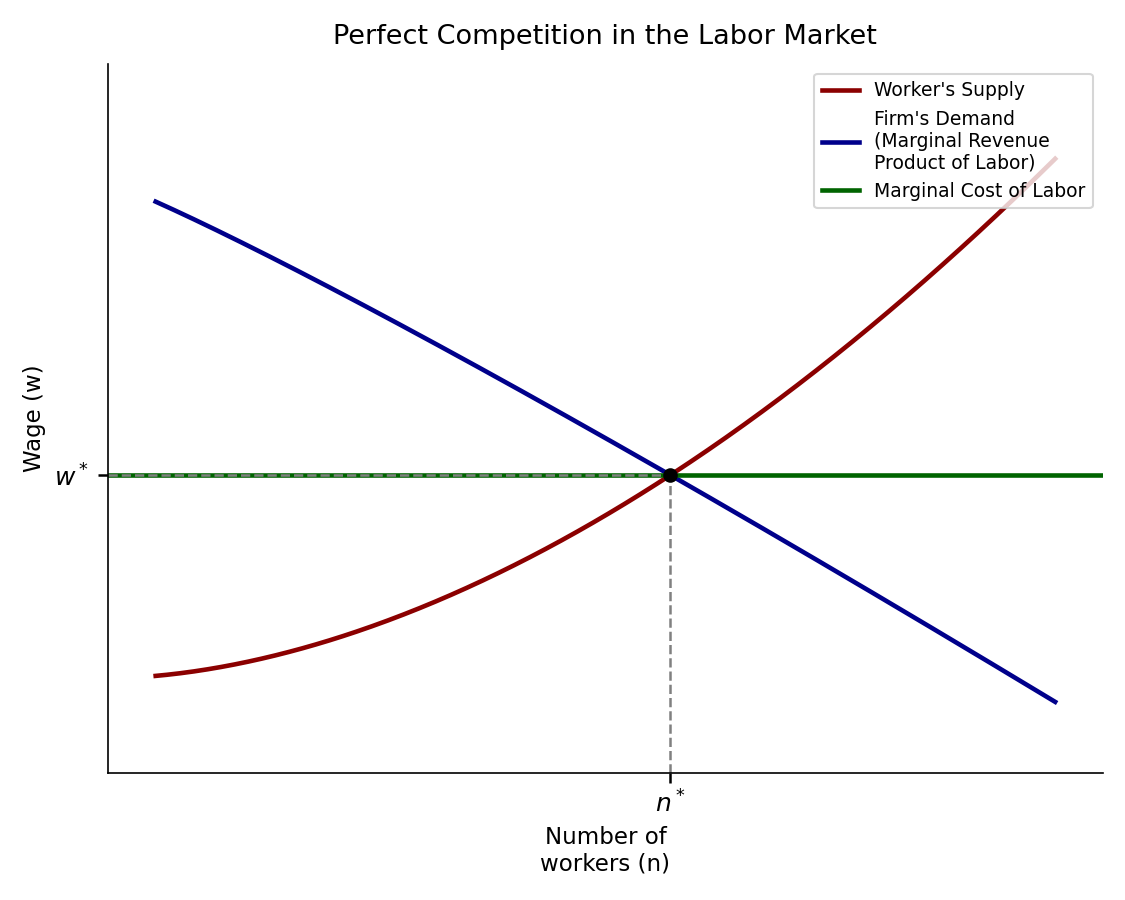
\includegraphics[width=\textwidth]{example_perfect_competition.png}
    \end{subfigure}
    \begin{subfigure}[b]{0.49\textwidth}
        \centering
        \caption{Monopsony}
        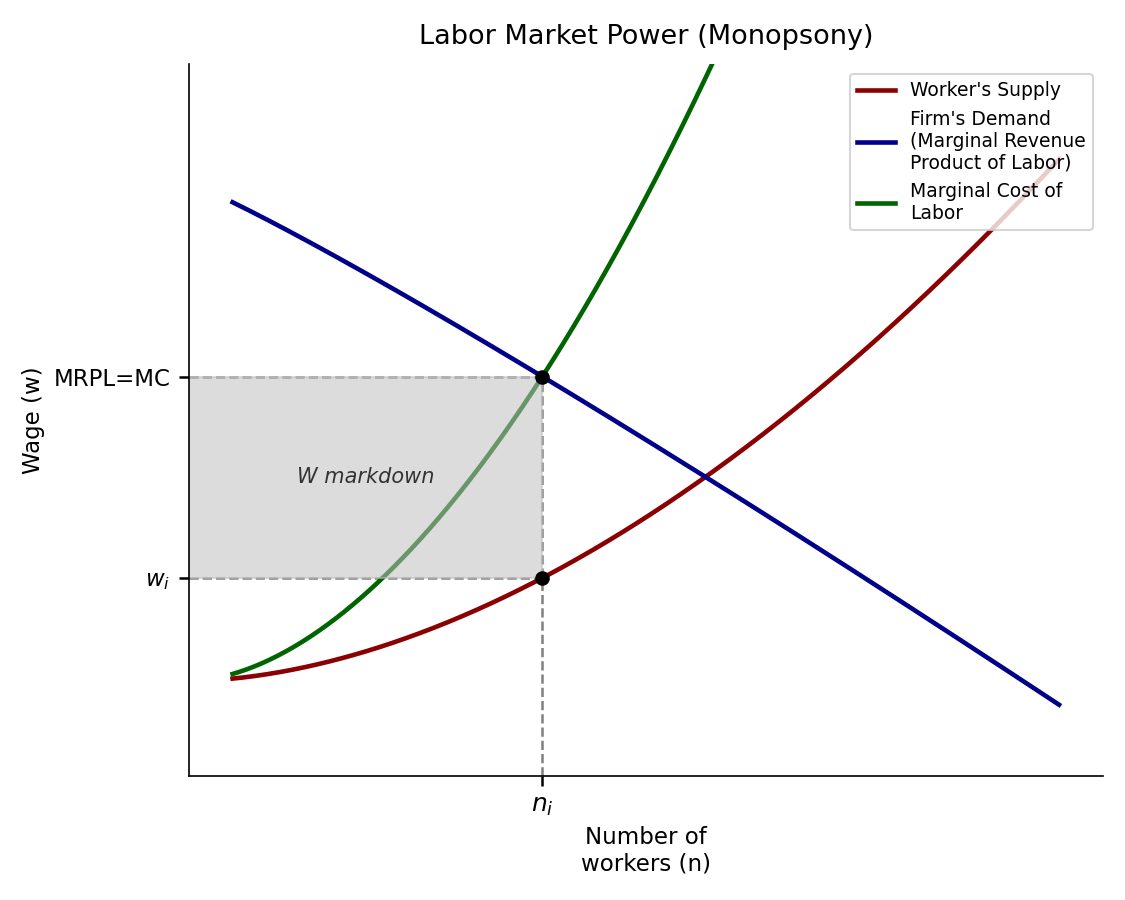
\includegraphics[width=\textwidth]{example_labor_marker_power.png}
    \end{subfigure}
\end{figure}

To understand how this markdowns arises, consider a firm's profit maximization problem with only one labor as input in a competitive market. The firm chooses labor input $L_{it}$ to maximize profits:

\begin{align}
\max_{L_{it}} \varPi_{it} = R_{it}(L_{it}) - \bar{w}L_{it},
\end{align}

Where $R_{it}(L_{it})$ is the firm's revenue as a function of labor input ($P*Q(L)$), and $\bar{w}$ is the constant wage in the competitive benchmark that the firm takes as given. The first-order condition for profit maximization equates the marginal revenue($R'(L)$) with the marginal cost ($W$) such that

\begin{equation}
\frac{\partial R_{it}(L_{it})}{\partial L_{it}} = \bar{w}
\end{equation}

For a monopsonistic firm, the wage is a function of the labor input $w_{it}(L_{it}) L_{it}$ reflecting the upward-sloping labor supply curve observed in figure \ref{fig:example}. The profit maximization problem becomes:

\begin{equation}
\max_{L_{it}} \varPi_{it} = R_{it}(L_{it}) - w_{it}(L_{it}) L_{it},
\end{equation}

The first-order condition for profit maximization

\begin{equation}
\frac{\partial R_{it}(L_{it})}{\partial L_{it}} = \frac{\partial w_{it}(L_{it})}{\partial L_{it}} L_{it} + w_{it}(L_{it}) 
\end{equation}

Note that the monopolistic firms also maximizes profits by equating marginal revenue and marginal cost, but the marginal cost of labor is greater than the wage in this case. The left hand side of the equation is the marginal revenue product of labor $\text{MRPL}_{it} \equiv \frac{\partial R_{it}(L_{it})}{\partial L_{it}}$, while the right-hand side is the marginal cost of labor, which includes both the wage paid to the marginal worker and the increase in wages paid to inframarginal workers. Factoring out the wage $w_{it}(L_{it})$ We can rewrite the equation as:

\begin{equation}
\text{MRPL}_{it} = \left(\frac{\partial w_{it}(L_{it})}{\partial L_{it}}{\frac{L_{it}}{w_{it}(L_{it})}} + 1\right)w_{it}(L_{it}) = \left(\varepsilon_{L}^{-1} + 1\right)w_{it}(L_{it}) 
\end{equation}

Where the firm's perceived inverse elasticity of labor supply is defined as:

\begin{equation}
\varepsilon_{L}^{-1} \equiv \frac{\partial w_{it}(L_{it})}{\partial L_{it}}{\frac{L_{it}}{w_{it}(L_{it})}}
\end{equation}

The markdown $\nu_{it}$ is then defined as the ratio of the marginal revenue product of labor to the wage:

\begin{equation}
\nu_{it} \equiv \frac{\text{MRPL}_{it}}{w_{it}(L_{it})} = \varepsilon_{L}^{-1} + 1,
\end{equation}

Under this definition, $\nu_{it} = 1$ under perfect competition (infinite labor supply elasticity) and $\nu_{it} > 1$ whenever labor supply is upward-sloping.

\section{Markdown Estimation - Production Approach}

From the theoretical framework, we see that the key parameter governing the size of the markdown is the firm's perceived labor supply elasticity $\varepsilon_L$. Nonetheless, estimating a firm's perceived elasticity of labor supply in a general setting is challenging, in part because of the potential for firm market power over both inputs (monopsony) and output (monopoly) \cite{yeh_monopsony_2022}. To disentangle these two forces, I follow \cite{yeh_monopsony_2022} and adopt the production approach of 
\cite{de_loecker_rise_2020}.

To understand this production approach, let's consider a Cobb-Douglas production function\footnote{For the actual estimation, following \cite{de_loecker_rise_2020} I use a translog production function with polynomial terms as follows:
%
\begin{equation*}
    \log(GO)_{it} = \beta_{0} + \beta_{1}\log(K)_{it} + 
    \beta_{2}\log(L)_{it} + \beta_{3}\log(M)_{it} + 
    \beta_{4}\log(K)^2_{it} + \beta_{5}\log(L)^2_{it} + 
    \beta_{6}\log(M)^2_{it} + \beta_{7}\log(K)_{it}\log(L)_{it} + 
    \beta_{8}\log(K)_{it}\log(M)_{it} + \beta_{9}\log(L)_{it}\log(M)_{it} 
    + t + e.
\end{equation*}} with three inputs --- labor $L_{it}$, capital $K_{it}$, and materials $M_{it}$ --- in an environment where the firm holds power over both its output and labor markets. Following \cite{de_loecker_rise_2020}, variable inputs ($L_{it}$, $M_{it}$) adjust frictionlessly within a period, while capital is subject to adjustment frictions.

The approach relies on the assumption that materials ($j = M_{it}$) is a fully flexible input satisfying three conditions: it incurs no adjustment costs within a period; its price is taken as given by the firm; and it is chosen statically, in the same period in which output is produced.

The firm's cost minimization problem is:

%
\begin{equation}
    \mathcal{L} = r_{it}K_{it} + w_{it}(L_{it})L_{it} + p^m_{it}M_{it} 
    - \lambda_{it} \left( P_{it}\bar{Q}_{it} - 
    A_{it}K_{it}^{\theta^K}L_{it}^{\theta^L}M_{it}^{\theta^M} \right)
\end{equation}
%

where $A_{it}$ denotes firm-specific productivity\footnote{Following \cite{de_loecker_rise_2020}, firm productivity is decomposed into a component observed by the firm but unobserved by the econometrician, modeled via an AR(1) process in which $A_{it} = A_{i,t-1} + \omega_t$. The component observed by the firm is $\omega_t$, the innovation in productivity.} and $\theta^K$, $\theta^L$, $\theta^M$ are the output elasticities of capital, labor, and materials, respectively. The price of capital is $r_{it}$, the wage function is $w_{it}(L_{it})$, and the price of materials is $p^m_{it}$. The Lagrange multiplier $\lambda_{it}$ captures the marginal cost of production.

The first-order conditions for $M_{it}$ and $L_{it}$ are:

\begin{equation}
\frac{\partial \mathcal{L}}{\partial M_{it}} = p^m_{it} - \lambda_{it} \varepsilon^M A_{it}K_{it}^{\theta^K}L_{it}^{\theta^L}M_{it}^{\theta^M-1}=0.
\end{equation}

\begin{equation}
\frac{\partial \mathcal{L}}{\partial L_{it}} = \frac{\partial w_{it}(L_{it})}{\partial L_{it}} L_{it} + w_{it}(L_{it}) - \lambda_{it} \varepsilon^L A_{it}K_{it}^{\theta^K}L_{it}^{\theta^L-1}M_{it}^{\theta^M}=0,
\end{equation}

We know from the theoterical framework that $\frac{\partial w_{it}(L_{it})}{\partial L_{it}} L_{it} + w_{it}(L_{it}) =\left(\varepsilon_{L}^{-1} + 1\right)w_{it}(L_{it})$. Also using the production function $Q_{it} = A_{it}K_{it}^{\theta^K}L_{it}^{\theta^L}M_{it}^{\theta^M}$, we can simplify the first-order conditions to:

\begin{equation}
p^m_{it} = \lambda_{it} \varepsilon^M \frac{Q_{it}}{M_{it}}
\end{equation}

\begin{equation}
\left(\varepsilon_{L}^{-1} + 1\right)w_{it}(L_{it}) = \lambda_{it} \varepsilon^L  \frac{Q_{it}}{L_{it}}
\end{equation}

Since $\lambda_{it}$ is the Lagrange multiplier on the production constraint, interpreted as marginal cost, the firm's markup---the price-to-marginal-cost ratio---is therefore:

%
\begin{equation}
    \mu_{it} = \frac{P_{it}}{\lambda_{it}}.
\end{equation}
%

Defining the revenue shares of labor and materials as:
%
\begin{equation}
    \alpha^L_{it} \equiv \frac{w_{it}(L_{it})L_{it}}{P_{it}Q_{it}}, 
    \qquad 
    \alpha^M_{it} \equiv \frac{p^m_{it}M_{it}}{P_{it}Q_{it}},
\end{equation}
%

substituting into the first-order condition for materials yields a markup estimator:

\begin{equation}
\mu_{it} = \frac{\theta^M}{\alpha^M_{it}},
\end{equation}

Substituting analogously into the first-order condition for labor gives:

\begin{equation}
\left(\varepsilon_{L}^{-1} + 1\right) = \frac{\theta^L}{\alpha^L_{it}} \frac{1}{\mu_{it}},
\end{equation}

Recalling from the theoretical framework that the markdown is defined as:
%
\begin{equation}
    \nu_{it} \equiv \frac{\mathrm{MRPL}_{it}}{w_{it}(L_{it})} = 
    \varepsilon_{L}^{-1} + 1,
\end{equation}
%
the markdown can be expressed in terms of observable quantities as:

%
\begin{equation}
    \nu_{it} = \frac{\theta^L}{\alpha^L_{it}} \cdot \frac{1}{\mu_{it}} 
    = \frac{\theta^L}{\alpha^L_{it}} \cdot \frac{\alpha^M_{it}}{\theta^M} 
    = \frac{\theta^L}{\theta^M} \cdot 
    \frac{p^m_{it}M_{it}}{w_{it}(L_{it})L_{it}}.
\end{equation}
%

This expression shows that the markdown can be estimated using the ratio of the firm's expenditure on materials to its wage bill, scaled by the ratio of output elasticities. The output elasticities $\theta^L$ and $\theta^M$ are estimated from the production function, while the input shares $\alpha^L_{it}$ and $\alpha^M_{it}$ are computed from observed data on wages, materials, output, and prices. This approach allows for the estimation of firm-level markdowns while controlling for both output and labor market power.

\section{Data}

This paper uses firm-level data from the Annual Manufacturing Survey (Encuesta Anual Manufacturera, EAM) conducted by the National Administrative Department of Statistics (DANE) in Colombia. The original dataset spans 1995-2024, covering approximately 7,000 manufacturing firms per year. The EAM is a census of medium and large manufacturing establishments and provides detailed and standardized information on firms' production, input use, employment composition, and financial accounts. I restrict the analysis to the period 2000-2019 to ensure data consistency and avoid disruptions from the COVID-19 pandemic. The data is collected at the plant level, nonetheless, I aggregate to the firm level by summing across all plants owned by the same firm in a given year, using the unique firm identifier provided in the dataset.

The data is organized as an unbalanced panel, reflecting firm entry and exit over time. Following DANE's technical guidelines, the sample is restricted to firms with at least 10 employees, which ensures consistency in reporting standards and improves the reliability of firm-level measures. Observations with missing or implausible values (e.g., negative output or extreme input ratios) are excluded (~0.2\% of total observations). 

The main explanatory variable is the share of female ownership at the firm level. This measure is constructed using variables c4r4c1t (number of male owners) and c4r4c2t (number of female owners)\footnote{In the form, these variables represent the total number of owners, partners, and unpaid family members. They are disaggregated by gender as well as by occupational category—professionals; technicians and technologists; production workers (foreign and local); operators and producers; and managers and sales personnel. I use the sum of all owner types to construct the total ownership variable.}. The female ownership share is defined as:
\begin{equation}
    \text{Female Ownership Share}_{it} = \frac{\text{Number of female owners}_{it}}{\text{Total number of owners}_{it}}.
\end{equation}
This variable ranges from 0 to 1 and captures the gender composition of firm ownership. Ownership is measured annually and may vary over time; firms with zero reported owners are excluded. One data limitation of this variable is that for only 30\% of firms, the number of owners is different from zero, which may reflect non-response or reporting issues. These observations are excluded from the analysis, which may introduce selection bias if the missingness is systematically related to firm characteristics or ownership structure. I will explore the extent of this potential bias in the data and consider robustness checks to address it.

The main outcome variable is the firm-level markdown, defined as the wedge between the marginal product of labor and the wage paid by the firm. Markdown estimates are obtained from the production function framework that combines estimated output elasticities with observed input shares; the construction is described in detail in the economic theoterical framework\footnote{I improved upon \cite{de_loecker_rise_2020} estimation procedure by using a Nelder-Mead primary optimizer, since the GMM surface can be non-smooth and non-convex, especially for the translog specification with its many cross-terms. Rvmmin (Variable metric nonlinear function minimization) provides a gradient-based refinement when Nelder-Mead stalls near the minimum. The estimation is run in a loop iterating over every distinct 4-digit ISIC sector in the data, with elasticities recovered at the firm level. For firms where the model did not converge, I follow  \cite{ackerberg_identification_2015} and use a Cobb-Douglas specification at the sector level, imputing the median sector-specific elasticities.}.

The dataset provides the necessary information to construct production function using the methodology by \cite{de_loecker_rise_2020}. Labor is measured as total employment, defined as the sum of permanent employees, firm owners, and temporary workers, both directly hired and outsourced. Capital is proxied by the book value of fixed assets, while the wage bill corresponds to total remuneration paid to permanent and temporary employees. Materials are measured as total expenditure on raw materials, intermediate inputs, and packaging, and are treated as the flexible input in production which also allows to control for unobservables (\cite{levinsohn_estimating_2003}). Gross output is proxied by firm-level total sales at factory's price without direct taxes as reported in the survey. The cost of capital is approximated using the user cost of capital formula, which incorporates the depreciation rate, interest rate, and inflation rate. The price of materials is calculated as the ratio of total material expenditure to the quantity of materials used.

All monetary variables are expressed in nominal Colombian pesos. The empirical analysis relies primarily on ratios and input shares constructed from these variables, which mitigates concerns related to price-level variation. In addition, the dynamic structure of the production function estimation implies that rescaling variables through deflation would not materially affect the estimation of key parameters.

Finally, the dataset includes detailed identifiers for industry (sector) and geographic location (region), which are used to control for heterogeneity in production technologies, input markets, and regional economic conditions.

The table \ref{tab:desc_stats} presents the descriptive statistics for the final dataset used in this analysis, it comprises of 7,849 Colombian manufacturing firms observed over 20 years (not balanced), covering 35,399 firm-year observations across 23 geographies and 104 industries. At the firm level, the average number of female owners is 0.66, with a mean female ownership share of 34.85\%, while male owners average 1.06 per firm. Firms employ an average of 37 workers, with wages per employee averaging \$1.87 thousand USD and mean gross output of \$1.61 million USD, though all these variables exhibit substantial dispersion, reflecting heterogeneity in firm size and performance. Production function estimates show that labor, capital, and materials have median output elasticities of 0.411, 0.074, and 0.545, respectively, with corresponding median output shares of 0.119, 0.043, and 0.478. Total Factor Productivity (TFP) has a median of 4.093, and pricing measures indicate a median markup of 1.124, a markdown of 3.029, and an inverse markdown of 0.330, suggesting variation in market power across firms. Overall, the data illustrate a diverse manufacturing sector with notable differences in ownership, size, productivity, and pricing behavior.

\begin{table}[!ht]
\centering
\caption{\label{tab:desc_stats}Descriptive Statistics}

\begin{tabular}{lrrrr}
\toprule
\multicolumn{5}{l}{\textbf{Overall}}\\
\midrule
\textit{Variable} & \textit{Value} & & & \\
\hspace{1em}Observations & 35,399 & & & \\
\hspace{1em}Years & 20 & & & \\
\hspace{1em}Firms & 7,849 & & & \\
\hspace{1em}Geographies & 23 & & & \\
\hspace{1em}Industries & 104 & & & \\
\midrule

\multicolumn{5}{l}{\textbf{By Firm}}\\
\textit{Variable} & \textit{Mean} & \textit{Min} & \textit{Max} & \textit{Std. Dev.}\\
\addlinespace[0.3em]
\hspace{1em}Female owners (N) & 0.66 & 0.00 & 58.00 & 0.89\\
\hspace{1em}Male owners (N) & 1.06 & 0.00 & 30.00 & 0.83\\
\hspace{1em}Female ownership share (\%) & 34.85 & 0.00 & 100.00 & 37.49 \\
\hspace{1em}Employees (N) & 37 & 1 & 4,025 & 108 \\
\hspace{1em}Wage per employee (\$ thousands USD) & 1.87 & 0.00 & 349.16 & 2.18\\
\hspace{1em}Gross output (\$ millions USD) & 1.61 & 0.00 & 3.21 & 21.49 \\
\midrule

\multicolumn{5}{l}{\textbf{By Firm -- Estimation Parameters}}\\
\textit{Variable} & \textit{p25} & \textit{Median} & \textit{p75} & \\
\addlinespace[0.3em]
\hspace{1em}Output elasticity of labor & 0.278 & 0.411 & 0.558 & \\
\hspace{1em}Output elasticity of capital & 0.037 & 0.074 & 0.118 & \\
\hspace{1em}Output elasticity of materials & 0.388 & 0.545 & 0.704 & \\
\hspace{1em}Total Factor Productivity (TFP) & 2.900 & 4.093 & 5.821 & \\
\hspace{1em}Labor output share & 0.070 & 0.119 & 0.190 & \\
\hspace{1em}Materials output share & 0.336 & 0.478 & 0.632 & \\
\hspace{1em}Capital output share & 0.020 & 0.043 & 0.088 & \\
\hspace{1em}Markup & 0.816 & 1.124 & 1.535 & \\
\hspace{1em}Markdown & 1.574 & 3.029 & 5.471 & \\
\hspace{1em}Inverse markdown & 0.183 & 0.330 & 0.635 & \\
\bottomrule
\end{tabular}

\caption*{\footnotesize Source: Author's calculations based on the Colombian Manufacturing Survey (EAM) 2000--2019. 
Note: The wage variable corresponds to the total wage bill of the firm divided by the number of employees, while gross output is proxied by total sales at factory price without direct taxes. The dollar values are calculated using an exchange rate of 1 USD = 3,670 COP. Output elasticities and input shares are estimated using the production function approach by \cite{de_loecker_rise_2020}. Markup and markdown estimates follow \cite{yeh_monopsony_2022}.}
\end{table}


In Figure \ref{fig:median_nu_l_inv}, I present the distribution of the inverse markdown by female ownership share, companies where the share is above 0, vs companies where there is no female ownership. The inverse markdown is defined as $\nu_{it}^{-1} = \frac{w_{it}(L_{it})}{\text{MRPL}_{it}}$. This transformation allows for a more intuitive interpretation, as higher values of the inverse markdown correspond to lower degrees of monopsony power. The figure shows that firms without female ownership (dummy=0) have a distribution more concentrated around lower values of the inverse markdown, suggesting that they tend to have pay employees with lower wages below their productivity compared to firms with at least one female owner (dummy=1).

\begin{figure}[!ht]
\centering
\caption{Distribution of Inverse Markdown by Female Ownership}
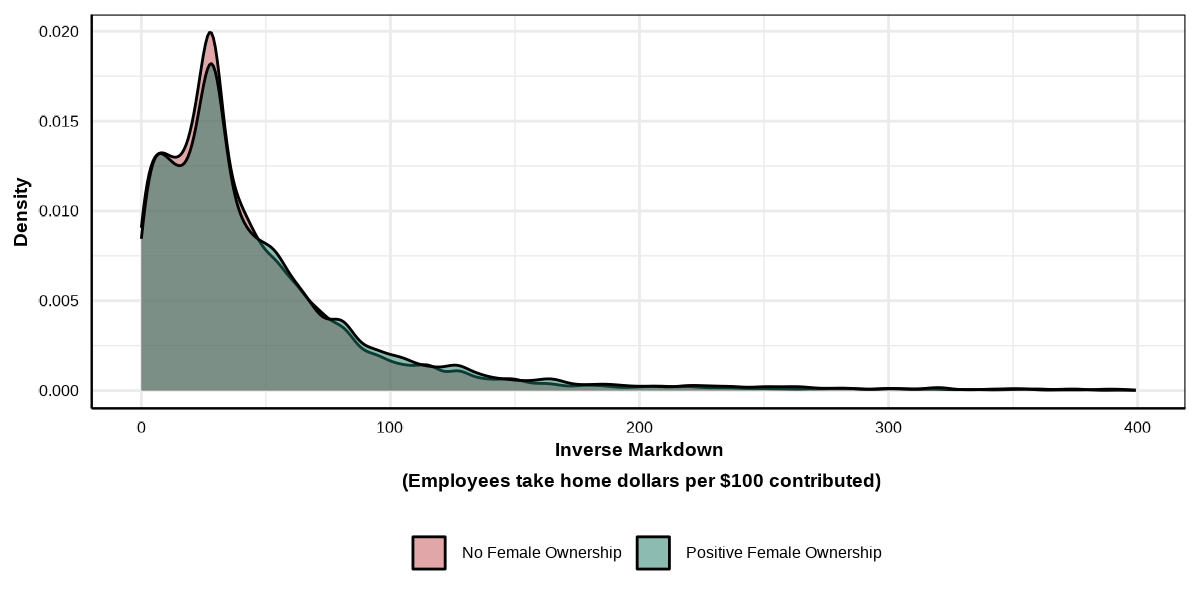
\includegraphics[width=1\textwidth]{distribution_nu_linv_female_dummy.png}
\source{Author's calculations based on the Colombian Manufacturing Survey (EAM) 2000--2019.}
\label{fig:median_nu_l_inv}
\end{figure}

\section{Empirical Framework}

To examine the relationship between female ownership and labor market power, I estimate the following linear regression:

\begin{equation}
\nu_{it} = \beta \, \text{Female}_{it} + \mathbf{X}_{it}'\boldsymbol{\gamma} + \alpha_t + \alpha_s + \alpha_r + \varepsilon_{it},
\label{eq:main}
\end{equation}

where $\nu_{it}$ is the inverse markdown for firm $i$ in year $t$. The outcome is expressed in levels so that $\beta$ has the interpretation of a absolute difference in markdowns between female-owned and male-owned firms, conditional on controls.

The main variable of interest, $\text{Female}_{it}$, measures the share of female ownership of the firm. The coefficient $\beta$ therefore captures the conditional association between female ownership and the firm's degree of monopsony power.

The vector $\mathbf{X}_{it}$ includes a set of firm-level controls. Firm age accounts for the possibility that older firms have had longer to build labor market power through reputation or search frictions. Firm size, measured by gross output, controls for scale effects on both the production side and the firm's capacity to set wages. Finally, I include the share of female workers and the share of skilled workers in the firm's workforce to account for differences in employment composition that may independently affect markdowns.

The specification includes three sets of fixed effects. Year fixed effects $\alpha_t$ absorb common macroeconomic shocks and aggregate trends in markdowns over time. Sector fixed effects $\alpha_s$ account for permanent differences across industries in production technology, product market structure, and average labor market competitiveness. Region fixed effects $\alpha_r$ control for local labor market conditions, including differences in the outside options available to workers. Standard errors are robust to account for heteroskedasticity.

The coefficient $\beta$ is identified from within-sector, within-region, within-year variation in female ownership across firms. The expected sign for the coefficient is $\beta < 0$ which would indicate that greater female ownership is associated with lower markdowns, consistent with female-owned firms exercising less monopsony power over their workers, conditional on observable firm characteristics.

\section{Preliminary Results}


\printbibliography
\end{document}